% Project-status slides -- anharmonic phonon quantum transport (quatrex).
% Numbers, the combined plots (fig/ratio_vs_T.pdf, fig/ratio_vs_L.pdf) and
% the status table are generated by   python make_slide_assets.py   from the
% production summaries; rerun it when new results land, then recompile.
% Figures resolve from ../fig/transport_sweeps and ./fig.
\documentclass[11pt,aspectratio=169]{beamer}
\usepackage{amsmath, amssymb, amsthm}
\usepackage{graphicx}
\usepackage{bm}
\usepackage{algorithm}
\usepackage{algpseudocode}
\usepackage{color}
\usepackage{tikz}
\usepackage{subcaption}
\usepackage{cleveref}
\usepackage{listings}
\usepackage{stmaryrd}
\usepackage{relsize}
\usepackage{physics}

% Theme settings
\usetheme{eth}

\colorlet{titlefgcolor}{ETHBlue}
\colorlet{accentcolor}{ETHPurple}

\title{Anharmonic Phonon Transport: Status}
\author{Paul Fischill}
\date{\today}

\setbeamerfont{footnote}{size=\tiny}

\newcommand{\vq}{\mathbf{q}}
\newcommand{\vk}{\mathbf{k}}
\newcommand{\qp}{\vq_{\!\perp}}
\newcommand{\kp}{\vk_{\!\perp}}
\newcommand{\ndof}{N_{\mathrm{DOF}}}
\newcommand{\nprim}{N_{\mathrm{p}}}
\newcommand{\Ncell}{N_{\mathrm{c}}}
\newcommand{\sse}[1]{\Sigma^{#1}}
\newcommand{\cO}{\mathcal{O}}
\newcommand{\Phit}{\tilde{\Phi}}

\lstset{
    stringstyle=\ttfamily,
    basicstyle=\footnotesize,
    showstringspaces=false
}

% headline numbers auto-generated from the production runs
\newcommand{\GenStamp}{2026-06-10 17:08}
\newcommand{\cntRatioLowT}{0.981}
\newcommand{\cntRatioRT}{0.878}
\newcommand{\cntTLow}{30}
\newcommand{\cntGballRT}{5.1}
\newcommand{\cntConsRT}{9e-05}
\newcommand{\cntLadder}{0.878 / 0.895 / 0.855}
\newcommand{\cntLadderL}{2/3/4}
\newcommand{\statCntThreeThree}{0.878 (300\,K) -- 9 pts (prod)}
\newcommand{\statCntEightZero}{0.775 (L1, 300\,K) (dense)}
\newcommand{\statSinwDFive}{0.942 (30\,K, $\lambda{=}0.3$) (dense)}
\newcommand{\statSinwDEleven}{0.997 ($\lambda{=}0.3$) (dense)}
\newcommand{\statSrtio}{running\dots}
\newcommand{\statSifilm}{0.52--0.38 (1.2--3.1\,nm) (dense)}
\newcommand{\ProdStatusRows}{%
    CNT(3,3) & 9 & 0.878 & done \\
    CNT(8,0) & -- & 0.775 & running \\
    SiNW d5a & -- & 0.942 & running \\
    SiNW d11a & -- & 0.997 & running \\
    SrTiO$_3$ & -- & -- & running \\
    Si film & -- & 0.52--0.38 & running \\
}


\begin{document}

\def\titlefigure{elements/title-page-image-alt}
% \titleframe

% -------------------------------------------------------------------
\begin{frame}{Anharmonic phonon NEGF: the 3-ph bubble in production}
\footnotesize
\begin{columns}[T,onlytextwidth]
\column{0.47\textwidth}
\textbf{SCBA 3-ph self-energy} (cubic FC $\Phi_{\mu\nu\nu'}$)
\[
\begin{aligned}
  \Pi^{\gtrless}_{\nu_{1}\nu_{4},\nu_{2}\nu_{3}}(\omega)
    &= \!\int\!\tfrac{\dd\omega'}{2\pi}\,
       G^{\gtrless}_{\nu_{1}\nu_{4}}(\omega')\,
       G^{\gtrless}_{\nu_{2}\nu_{3}}(\omega{-}\omega') \\[4pt]
  \sse{\gtrless}_{\mu\mu'}(\omega)
    &= \tfrac{i\hbar}{2}\!\!\sum_{\nu_{1}\nu_{2}\nu_{3}\nu_{4}}\!\!
       \Phi_{\mu\nu_{1}\nu_{2}}\,
       \Pi^{\gtrless}_{\nu_{1}\nu_{4},\nu_{2}\nu_{3}}(\omega)\,
       \Phi_{\mu'\nu_{3}\nu_{4}}
\end{aligned}
\]
\medskip
convolution evaluated as a $\tau$-product:
\[
  \Pi^{\gtrless}(\omega)=\mathcal{F}^{-1}\!\big[\,g^{\gtrless}(\tau)\,g^{\gtrless}(\tau)\,\big]
\]
\medskip
3 MPI axes\;\; $P = P_{\omega}\times P_{\mathrm{blk}}\times P_{\qp}$
\\[2pt]
{\scriptsize (energy $\times$ device blocks $\times$ transverse $\qp$)}

\column{0.49\textwidth}
\textbf{Production pipeline} (\texttt{src/quatrex})

\smallskip
two layouts: \textbf{stack} (split $\omega$, full matrix)
$\rightleftarrows$ \textbf{nnz} (split elements, full band)

\smallskip
\begin{enumerate}\setlength{\itemsep}{3pt}\setlength{\leftmargini}{1.4em}
  \item FFT $G(\omega)\!\to\! g(\tau)$ \hfill [nnz]
  \item \texttt{dtranspose} nnz$\to$stack \hfill {\scriptsize all-to-all over $\omega$}
  \item ring $\sse{\gtrless}(\tau)=\Phi\,[g\,g]\,\Phi$ \hfill [stack]
    \\[1pt] {\scriptsize \emph{halo exchange} of band links across
    \texttt{comm.block} neighbours}
  \item \texttt{dtranspose} stack$\to$nnz
  \item IFFT $\sse{\gtrless}(\tau)\!\to\!\sse{\gtrless}(\omega)$ \hfill [nnz]
\end{enumerate}
\end{columns}
\end{frame}

% -------------------------------------------------------------------
\begin{frame}{CNT: channel freezing and length ladder (production)}
\footnotesize
\begin{columns}[T,onlytextwidth]
\column{0.36\textwidth}
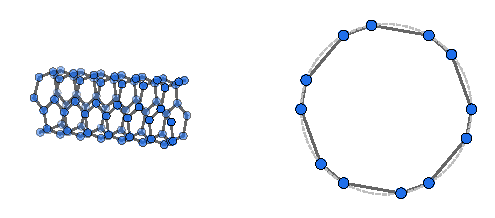
\includegraphics[width=\linewidth]{fig/cnt_structure.pdf}

\smallskip
{\scriptsize
\begin{itemize}\setlength{\itemsep}{2pt}\setlength{\leftmargini}{1.1em}
  \item CNT(3,3): $G_{\mathrm{anh}}/G_{\mathrm{ball}}$
    \textbf{0.98$\rightarrow$0.89} (30$\rightarrow$300\,K) ---
    ballistic limit as channels freeze (a)
  \item length ladder + CNT(8,0): onset of the resistive regime;
    $L\,{\ge}\,4$ only with the distributed solver (b)
  \item anharmonic shifts spectral weight to low-$\omega$ acoustic
    modes (c,d)
\end{itemize}}

\smallskip
{\scriptsize Same physics, other methods: ballistic$\to$diffusive
(Wang \& Wang, APL \textbf{88}, 2006); zigzag 3-ph Umklapp (Xiao
\emph{et al.}, JPCM \textbf{15}, 2003); ph--ph linewidths (De~Martino
\emph{et al.}, PRB \textbf{79}, 2009).}

\column{0.63\textwidth}
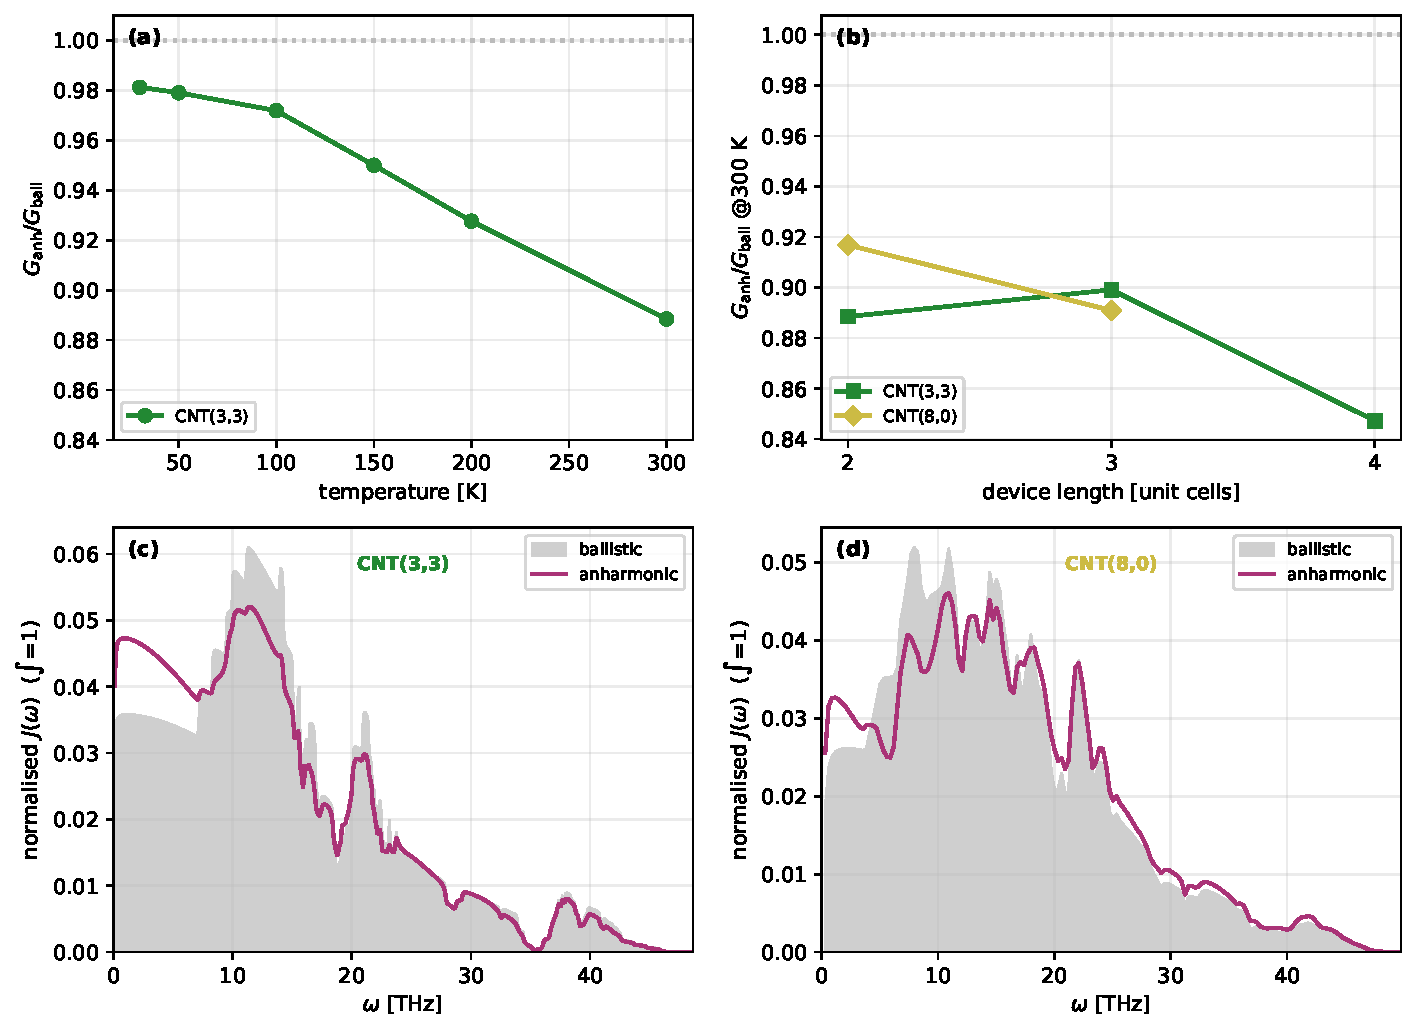
\includegraphics[width=\linewidth]{fig/cnt_prod.pdf}
\end{columns}
\end{frame}

% -------------------------------------------------------------------
\begin{frame}{Silicon Nanowires}
\footnotesize
\begin{columns}[T,onlytextwidth]
\column{0.52\textwidth}
\[
\begin{aligned}
  \sse{\mathrm{tad}}_{\mu\mu'} &= -\tfrac{i}{2}\!\!\sum_{\nu\nu'\kappa\lambda}\!\!
    \Phi_{\mu\mu'\nu}\,(\Phi_{\mathrm{eff}}^{+})_{\nu\nu'}\,\Phi_{\nu'\kappa\lambda}
    \!\int_{\omega}\! G^{<}_{\kappa\lambda} \\[4pt]
  \sse{\mathrm{loop}}_{\mu\mu'} &= \tfrac{i}{2}\sum_{\kappa\lambda}
    \Phi^{(4)}_{\mu\mu'\kappa\lambda}\!\int_{\omega}\! G^{<}_{\kappa\lambda} \\[4pt]
  \Phi_{\mathrm{eff}} &= D + \sse{\mathrm{tad}} + \sse{\mathrm{loop}}
\end{aligned}
\]
\vspace{-4pt}
{\scriptsize $\int_{\omega}\!\equiv\!\int\!\tfrac{\dd\omega}{2\pi}$;\;
$\Phi_{\mathrm{eff}}^{+}$ = pseudo-inverse over the \emph{stiff optical} modes
($G^{R}(\omega{\to}0)$ diverges as $1/\omega^2$ on the acoustic/soft modes).}
\begin{itemize}\setlength{\itemsep}{3pt}
  \item small NW has soft 0.0075\,THz mode, very difficult to get to converge
   \item loop is the largest correction, still low conservation
  \item diagonal-$G$ approximation off by $5$--$30\times$
\end{itemize}

\column{0.46\textwidth}
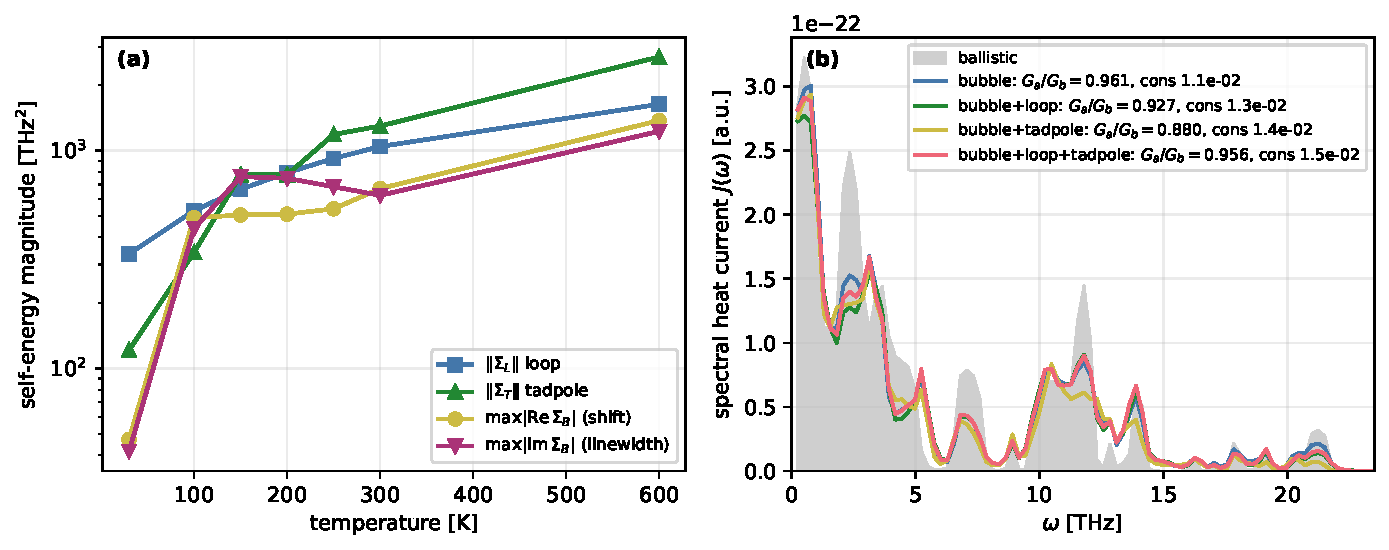
\includegraphics[width=\linewidth]{fig/static_se_replot.pdf}
\end{columns}
\end{frame}
% -------------------------------------------------------------------
\begin{frame}{Si thin film}
\footnotesize
\begin{columns}[T,onlytextwidth]
\column{0.50\textwidth}
\[
  \sse{\gtrless}(\qp,\omega) = \sum_{\qp'}
    \Phit(\qp',\qp{-}\qp')\,
    \big[G^{\gtrless}(\qp')\,G^{\gtrless}(\qp{-}\qp')\big]\,
    \Phit^{\dagger}
\]
\begin{itemize}\setlength{\itemsep}{3pt}
  \item $\qp'$-convolution couples all transverse momenta
  --- needs a formulation that scales to large systems
  \item ballistic: $2^3$ supercell FC reproduces Guo's scale (a);
    the larger, converged supercell softens FC2
  \item anharmonic reduction grows with thickness (diffusive),
    ${\sim}50$--$60\%$; $2^3$ and large FC3 agree (b)
  \item larger than Guo's ${\sim}10$--$20\%$: the coupled-$\qp$
    NEGF captures more scattering
\end{itemize}

\column{0.46\textwidth}
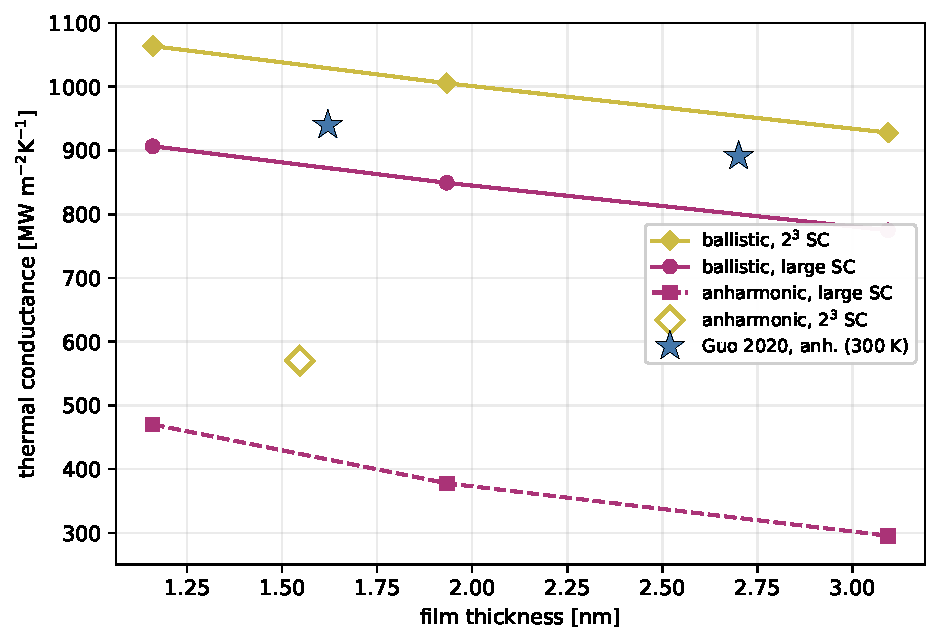
\includegraphics[width=\linewidth]{fig/si_film_prod.pdf}
\end{columns}
\end{frame}

% -------------------------------------------------------------------
\begin{frame}{SrTiO$_3$: the AFD soft mode --- two routes}
\footnotesize
\begin{columns}[T,onlytextwidth]
\column{0.50\textwidth}

\includegraphics[width=0.97\linewidth]{fig/srtio3_rattle_renorm.pdf}

\smallskip
{\scriptsize Large-amplitude (high-displacement) effective FC2 lifts the
unstable AFD soft mode at $M$/$R$ --- the same renormalisation the
loop+tadpole static self-energy provides diagrammatically.}

\smallskip
{\tiny T.~Tadano, S.~Tsuneyuki, JPSJ \textbf{87}, 041015 (2018).}

\column{0.46\textwidth}
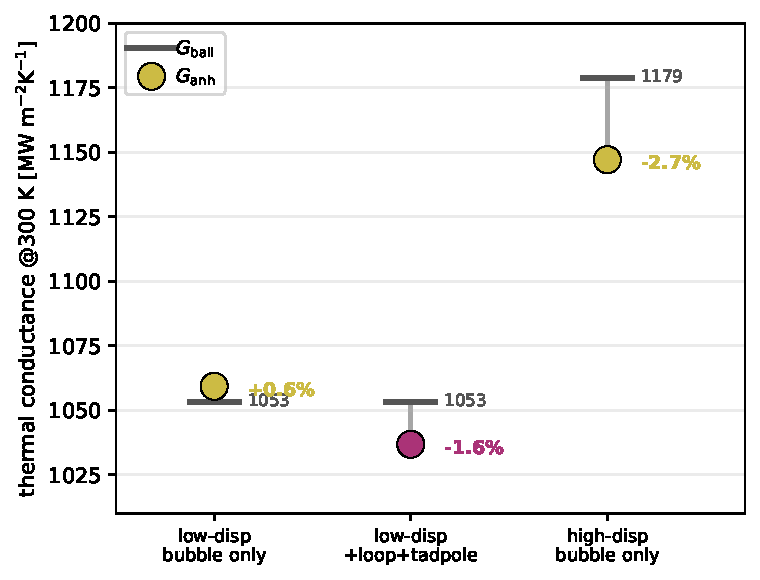
\includegraphics[width=\linewidth]{fig/srtio3_transport.pdf}

\smallskip
{\scriptsize
\begin{itemize}\setlength{\itemsep}{2pt}\setlength{\leftmargini}{1.1em}
  \item the high-disp effective FC2 \emph{shifts} $G_{\mathrm{ball}}$
    ($1053{\to}1179$) --- so a cross-route \emph{ratio} is misleading;
    compare the $G_{\mathrm{ball}}{\to}G_{\mathrm{anh}}$ drop at each FC
  \item bubble-only on \emph{low}-disp FCs: $+0.6\%$ (soft mode not
    captured); \textbf{loop+tadpole (SCP) needed} $\Rightarrow -1.6\%$
    (converged, FC4)
  \item high-disp bubble-only: $-2.7\%$ --- same scattering once the FC2
    is renormalised
\end{itemize}}
\end{columns}
\end{frame}

\end{document}
